\section{APPENDIX A - MORE DETAILS}

\subsection{Brief context of Time Operators}
\label{ap:time_context}

In early quantum theory, time was treated as an external classical parameter, rather than a quantum observable. Unlike the position operator $\hat{x}$ or the momentum operator $\hat{p}$, time doesn't currently have an adequate self-adjoint \textbf{time operator} in quantum formalism. Historically, Wolfgang Pauli has formulated this asymmetry with \textbf{Pauli's No-Go Theorem} (1933), stating that if a time operator $\hat{T}$ would exist that is canonically conjugate to the Hamiltonian $\hat{H}$, satisfying the commutation relation

\begin{align}
    [\hat{T}, \hat{H}] = i\hbar
\end{align}

then the spectrum of the Hamiltonian must span the entire real domain, with the implication that the spectrum is \textbf{unbounded} both above and below, meaning that there would be no maximum nor minimum energy in the spectrum. For bounded particle this implies that they could exhibit arbitrarily negative energies, which contracts real-world systems that have empirically a measurable ground state. For Free particles on the other hand, with $\hat{H}=\frac{\hat{p}^2}{2m}$, are defined only for non-negative energies (these are bounded below), which correspond to observations in laboratories, and thus violate the consequences of Pauli's No-Go Theorem \cite{book:wolfgangpauli} \cite{paper:paulitheorem}.
\\\\
Neither in literature, nor on Reddit, have an adequate and satisfactory time operator has been published or suggested thus far. However, under modern treatments it is possible to produce non-self adjoint operators which \textit{act} like time operators. This usually involves careful considerations of highly specific cases, rather than generalizations \cite{paper:paulitheorem}. Introducing quantum clocks, as part of the considered Hamiltonian system, through so called PWAK mechanisms \cite{paper:quantumclocks} also seem to circumvent the limitations paused by Pauli's Theorem. Modern approaches involve analysis and simulations of \textbf{Positive Operator-Valued Measures} (POVMs), which are suitable for outputting strictly positive probability distributions.
\\\\
Their analysis usually involves considerations of quantum mechanical probability currents like in \cite{paper:probability_current}, or using absorbing boundaries like in \cite{paper:tumulka}.

\subsection{Arrival Time and Tunnelling Time in Free Fall Experiments}
\label{ap:arrivaltimetunnelingtime}

Even though an adequate \textbf{Time Operator} has not yet been produced, characteristic times of experiments are being measured routinely in laboratories (see table \ref{tbl:characteristic_times}). In this paper, focus has been put on asking the following central question:
\begin{center}
    \textit{When will a detector click?}
\end{center}
The answer to this question is answered by the production of an \textbf{arrival time} distribution for a given setup. Of course, physics heralds its predictive and powerful legacy in both theoretical prediction and experimental verification. When no barriers or potentials are present in the time evolution of a quantum mechanical system, semi-classical approaches are exceedingly accurate for predicting the probability of arrival time \cite{paper:semiclassical}. In this paper, however, tunnelling and potential barriers are taken into consideration.
\\\\
Perhaps most importantly, one ought to take the initial conditions of particles into consideration - the initial position and momentum of a particle have an inherent spread due to the uncertainty principle, making the arrival time inherently ambiguous. This is especially the case when \textit{shooting} particles, as is done in most experiments.
\\\\
For precise measurements of the arrival time, one way to tackle this is to consider a \textbf{physically realizable experiment} where \textbf{a particle in rest is released in free fall onto a barrier}. A detector is placed below the barrier. In this setup, the particle will fall onto the barrier, part of it will reflect, and another part will transmit. The reflected portion of the particle will fall back onto the barrier due to linear gravitational potential. See figure \ref{fig:1d_setup} on page \pageref{fig:1d_setup} for the setup of this experiment. When considering a delta barrier in specific far-field regimes, the arrival time can be approximated via the probability current, this is further discussed and argued in the theory section ahead, which has a Bohmian Mechanical justification for it.\\\\
\fbox{%
  \begin{minipage}{0.45\textwidth}
  The expected arrival times of particles falling onto gaussian barriers under free fall has not yet been conducted, making this study an initial theoretical analysis of such setups
  \end{minipage}%
}
\\\\
Even though this will be explicated later in the theory section, it's interesting to note ahead that the Broglie-Bohm Pilot Wave Theory, or shortly \textbf{Bohmian Mechanics}, makes exactly the same predictions as the wave function formalism of quantum mechanics, but poses that quantum particles are dot like entities which follow a well-defined pathway, guided by a pilot wave (or quantum potential Q). Since the predictions are 1-to-1 with the canonical wave function formalism, the realism aspect of Bohmian Mechanics become interesting insofar as being unambiguous when considering the arrival time of quantum particles. Even more shockingly, it seems that Bohmian Mechanics poses the only unambiguous solution towards answering the question of arrival time, even though it's generally not accepted in canonical quantum formalism \cite{Das2019}.
\\\\
A second central question considered in the study is

\begin{center}
    \textit{How long does a particle spend in a barrier?}
\end{center}

The answer to this question is answered by the prediction and measurement of \textbf{tunnelling time}. For a substantial period, physicists have considered barrier time to be superluminal (being faster than light). For instance, in 1980s the discussion has shifted to the consideration of "interaction time" of a particle with a barrier. Experiments have shown that \textit{group delay} (phase time, or Wigner Time) \textbf{is} in fact superluminal in nature, however tunnelling time itself has been measured to be finite \cite{paper:tunneling_atom}. Ramos et Al in \cite{paper:tunneling_atom} have studied this by tunnelling Bose-condensed $^{87}Rb$ atoms through a $1.3 \mu m$ optical barrier. By measuring \textbf{Larmor spin precession} of spin-$\frac{1}{2}$ particles through this barrier, via the clasically derived Larmor Frequency $\omega_L$, they arrived a tunnelling time as a derived quantity, and hence the time it took for the particle to cross the clasically forbidden region. The measurement of spin precession usually involves setting up Stern-Gerlach experiments after passing a barrier. This approach is often called the \textbf{Larmor Clock} approach in literature, which is a classical approach to a quantum mechanical regime.
\\\\
In this paper, the Larmor Clock approach is compared with predictions made by Bohmian Theory by means of numerical simulations, since the TDSE is analytically unsolvable but for the most basic potentials \cite{book:cohen_qm} \cite{book:griffiths_qm}. The \textbf{tunnelling time $\tau_\text{tunnelling}$} predicted by the two approaches are compared, analyzed, and scrutinized. The two theoretical frameworks are analysed on first principles basis as well in the discussion section. For simplicity of setup, this last approach is similar to the aforementioned setup: a particle (spin-$\frac{1}{2}$ this time) in rest is dropped in free fall, onto a \textbf{uniform magnetic barrier}. The expectation values of Pauli Spinors $\langle\sigma_x\rangle$ and $\langle\sigma_y\rangle$ are calculated and transformed into a spin precession calculation. This value for \textbf{tunnelling time} is compared to what a \textbf{bohmian view} would predict by the calculation of bohmian trajectories for the same quantum particle in the same setup through a magnetic barrier. The bohmian tunnelling time is numerically by following the guiding pilot wave $Q$ throughout the barrier.
\\\\
The following theory section will expand on theoretical ideas and frameworks, including methods for numerically simulation of quantum mechanical systems.

\begin{table*}[t] % or [b] for bottom
\centering
\caption{Characteristic times}
\begin{tabular}{lll}
\hline
\textbf{Time} & \textbf{Name} & \textbf{Description} \\
\hline
\label{tbl:characteristic_times}
$\tau_L$ & Lifetime & Usual lifetime for decay, $\hbar/2\pi\rho(E)|\langle f|H|i\rangle|^2$ \\
$\tau_Z$ & Zeno time & Inverse of energy spread, $\hbar/\sqrt{\langle \psi | (H - E_\psi)^2 | \psi \rangle}$ \\
$\tau_J$ & Jump time & $\tau_Z^2/\tau_L$ \\
$\tau_T$ & Tunnelling time & Time spent in barrier \\
$\tau_A = \Pi$ & Arrival time & Time of arrival at a detector \\
$\tau_P$ & Passage time & Minimum time to go from a state to a $\perp$ one, $\pi\tau_Z/2$ \\
$\tau_R$ & Response time & A property of monitoring apparatus \\
$\tau_{PM}$ & Pulse time & Interval between ideal pulsed measurements (cf. QZE) \\
$\tau_{\text{Door}}$ & Door time & Metaphorical \\
\hline
\end{tabular}
\end{table*}

\subsection{Arrival Time}
\label{ap:arrivaltime}

This section starts by considering the arrival time in quantum mechanical systems, the explanation is adapted from \cite{paper:probability_current}, omitting the semi-classical approach in this discussion. The discussion starts with the canonical quantum formalism, after which the shift towards Bohmian mechanics is made.

\subsubsection{Arrival Time From a Canonical Perspective}

Consider a particle that crosses a detector at time \textit{t'} with 100\% certainty. This implies that the particle was on one side of the detector before $t'$, and on the other side after $t'$, which leads to a good reason to connect arrival time statistics with the probability that a particle is on one side of the detector at different times. Consider the easiest possible case, depicted in figure \ref{fig:ideal_situation}, a one dimensional free particle is placed on the positive real half-line, moving towards the origin, with strict negative momentum:

\begin{align}
    \psi_0(x, t=0) \approx 0 && \forall x \leq 0\\
    \tilde{\psi}_0(p, t=0) = 0 && \forall p \geq 0
\end{align}

\begin{figure}
    \centering
    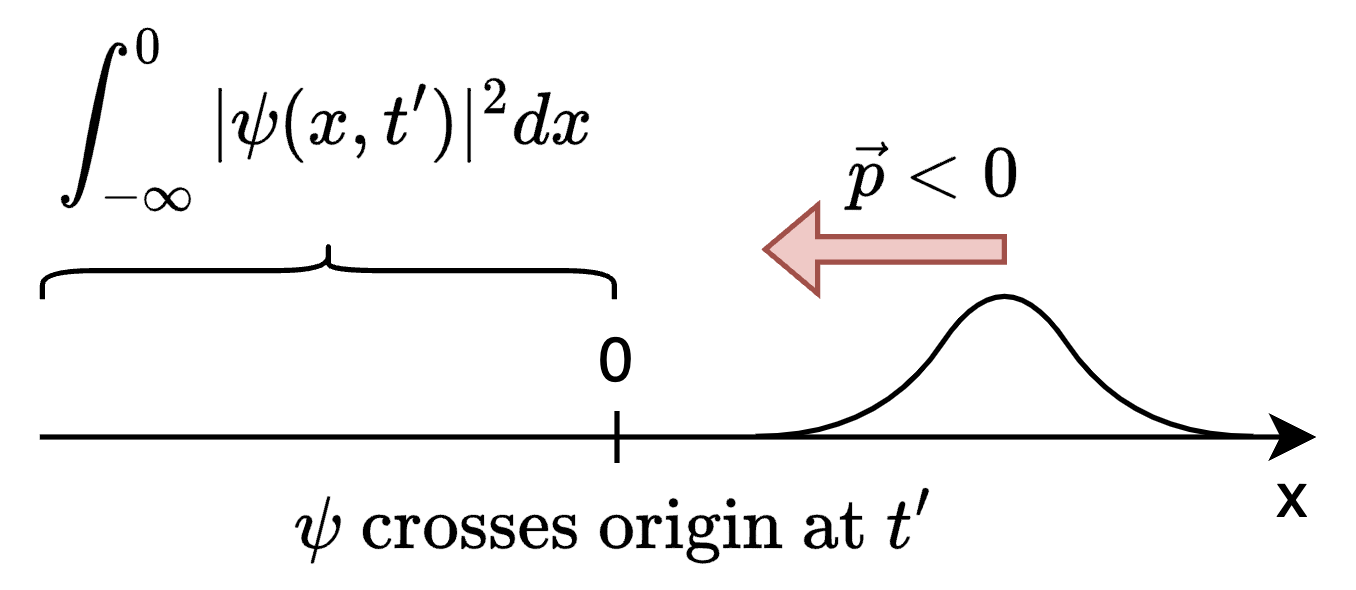
\includegraphics[width=1\linewidth]{Figures/ideal_situation.png}
    \caption{A simple setup for discussing arrival time. The particle has a strictly negative momentum and moves towards the origin where a detector sits}
    \label{fig:ideal_situation}
\end{figure}

With $\tilde{\psi}$ the Fourier transformed of $\psi_0$. Having a strict negative momentum, the particle is guaranteed to cross the origin, and thus cross the detector from right to left. In this situation, having the particle cross the origin at time $t'$, it's not far-fetched to think that the probability to have the particle cross the origin at a time $\tau > t'$, is the probability of finding the particle still in the positive region at time $t'$:

\begin{align}
    P(\tau \geq t') &= P(x \geq 0, t=t') \\
    &= \int_0^{\infty} |\psi(x, t=t')|^2 \space dx
\end{align}

On the other hand, the probability to have the particle cross the detector before $t'$ is:
\begin{align}
    P(\tau < t') &= 1- P(\tau > t')\\
    &= \int^0_{-\infty} |\psi(x, t=t')|^2 \space dx
\end{align}
Hence, the probability density $\Pi(t)$ for crossing the detector at time $t$ is given by, substituting $t' \rightarrow t$:

\begin{align}
    \label{eq:init}
    \Pi(t) &= \frac{d}{dt} P(\tau < t) \\
    &= \int^0_{-\infty} \frac{\partial}{\partial t} \space |\psi(x,t)|^2 \space dx
\end{align}

Because solutions to the schrödinger equation are subject to the \textbf{probability continuity equation,} which states that:

\begin{align}
    \frac{\partial}{\partial t} |\psi(x,t)|^2 + \frac{\partial}{\partial x} j(x,t) = 0
\end{align}

with $j(x,t)$ the probability current defined as:

\begin{align}
    \label{eq:continuitity_1}
    j(x,t) = \frac{\hbar}{m} \Im \left( \psi^* \frac{\partial}{\partial x} \psi \right)
\end{align}

Equation \ref{eq:continuitity_1} can now be substituted into equation \ref{eq:init} giving

\begin{align}
    \label{eq:continuitity_1}
    \Pi(t) &= \frac{d}{dt} P(\tau < t) \\
    &= - \int^0_{-\infty} \frac{\partial}{\partial x} j(x,t) \space dx \\
    &= - j(x=0, t) + j(x= -\infty, t)\\
    &= - j(x=0, t)
\end{align}

This gives the following result:

\fbox{%
  \begin{minipage}{0.45\textwidth}
  The probability density of the arrival time $t$ at a detector in the origin, is given by the probability current at the origin.
  \begin{align}
    \label{eq:continuitity_1}
    \Pi(t) = - j(x=0, t)
    \end{align}
  \end{minipage}%
}

The boxed result only works when the \textbf{probability current is strictly negative, which cannot be generally guaranteed,} even though the momentum was strictly negative in the setup. A strictly negative momentum implies that the momentum would be measured strictly negative. Before measurement there's no sense of speaking of a particle's position, nor momentum, therefore there's no way of conceiving how a particle moves in the system in this framework. In canonical quantum formalism, it's unwarranted to claim that a particle will only \textit{moves one time} from the negative real-line to the positive real-line. In literature, the issue of having no strictly negative (or positive when considering flow in the positive direction) the issue of having no \textbf{backflow}. In fact, up the moment of writing, no adequate POVM $\hat{O_t}$ (a superset of usual projection-valued measures (PVMs) in quantum mechanics) has been constructed as to produce a strictly positive probability arrival distribution \cite{MUGA2000353}. Even worse, it has been demonstrated that no general POVM $\hat{O}$ exists for which the following holds \cite{Vona_2013}:
\begin{align}
\langle \psi_0 | \hat{O_t} | \psi_0 \rangle = j(x=0, t)
\end{align}
In other words, canonical quantum mechanics is foremost a framework for \textit{predicting measurement outcomes}, and therefore, quantum mechanical quantities are not intrinstic parts of the system under study, or independent of the measurement device.

\subsubsection{Entering Bohmian Mechanics}

Bohmian Mechanics is an alternative theory of quantum phenomena, yet giving the same emperical predictions as canonical quantum mechanics \cite{DurrTeufel2009} \cite{DurrGoldsteinZanghi2013}. Both theories share their foundations in the concept of a wave function which obeys the Schrödinger equation. Canonical quantum mechanics has some further postulates regarding the collapse of the wave function, and how all objects are described by wave functions. Bohmian Mechanics poses that the world around us is composed of real point particles that move alongside continuous pathways, also called \textbf{bohmian trajectories}, guided by a guidance wave or \textbf{pilot wave}. The latter is determined by the wave equation. The usual quantum mechanical formalism can be recovered from Bohmian mechanics as an effective descritpion of measurement situations.
\\\\
It's important to state that canonical quantum theory is concerned with \textbf{measurement outcomes} whereas Bohmian Mechanics gives an account of the physical reality in a quantum setup. In other words, canonical quantum theory deals with PVMs and POVMs exclusively, whereas even though Bohmian mechanics predicts the same outcome, they're not the main focus of the bohmian view.
\\\\
In non-relativistic quantum mechanics, a general wave function can be written as

\begin{align}
    \Psi = \sqrt{\rho(\vec{r},t)} \cdot \text{exp}\left( i \frac{S(\vec{r},t)}{\hbar} \right)
\end{align}

Where $\rho(\vec{r},t) = \Psi^*\Psi$ the probability density of the wave function, and $S(\vec{r},t)$ its phase. In Bohmian Mechanics, particle are real (they don't span the whole space) and are \textit{guided} by a \textbf{guiding equation} or \textbf{pilot wave}. This guiding equation determines a well-defined velocity for every particle passing through a velocity field of the following form:

\begin{align}
\label{eq:velocityfield}
\vec{v} = \frac{\vec{j}(\vec{r}, t)}{\rho(\vec{r}, t)} = \frac{1}{m} \nabla S(\vec{r},t)
\end{align}

Where $\vec{j}$ represents the probability current or \textbf{probability flux} of the wave function. The spatial variation of the wave function characterizes the probability flux of the wave function, and thus also its velocity. Having the velocity equal to $\frac{\nabla S(\vec{r},t)}{m}$ is interestingly a classical limit in fluid dynamics.
\\\\
The arrival time of a particle in Bohmian Mechanics can be determined by following the motion of a particle's Bohmian trajectory, then registering the time at which the trajectory arrives at detector:
\begin{align}
\frac{d}{dt} \vec{r}(t) = \vec{v} (\vec{r}(t), t) = \frac{|j(\vec{r}(t), t)|}{|\Psi(\vec{r}(t), t)|^2} \\
\Rightarrow \vec{r} = \vec{r}_0 + \int_0^t \vec{v} dt
\end{align}

The Bohmian Mechanical velocity of a particle in her domain is not directly related to the quantum mechanical momentum, rather it encodes information about the possible results of possible momentum measures. To obtain the same predictions as canonical quantum mechanics, one ought to \textit{spawn} or start sufficient Bohmian particles at $t=0$, in a probability distribution that is in accordance with $|\psi(x,t=0)|^2$, then averaging the arrival times (or arrival positions) across all particles in the ensemble.
\\\\
The arrival time $\Pi(t)$ can now be interpreted in light of Bohmian Mechanics. Previously, the requirement was to have the momentum of the particle be strictly negative (as in: moving towards the origin from the positive real axis). Now, we require the Bohmian velocity to stay negative after the initial state preparation. When a particle crosses a detector at $x=0$, the trajectories would have spanned a distance $\vec{v}(x=0,t)dt$ in a timespan $t+dt$ (see figure \ref{fig:probability_current_dt}). This probability to arrive in this region beyond the detector is the distance covered ($\vec{v}(x=0,t)dt$) multiplied by the probability to find a particle there, $|\psi(x=0,t)|^2$, which gives a simple equation for the arrival time distribution, with the minus put in place since we're considering negative velocities in the discussed setup:

\begin{align}
    \Pi(t) &= - \frac{d}{dt} |\psi(x=0,t)|^2 \space \vec{v}(x=0,t) \space dt\\
    &= - j(x=0, t)
\end{align}

\begin{figure}
    \centering
    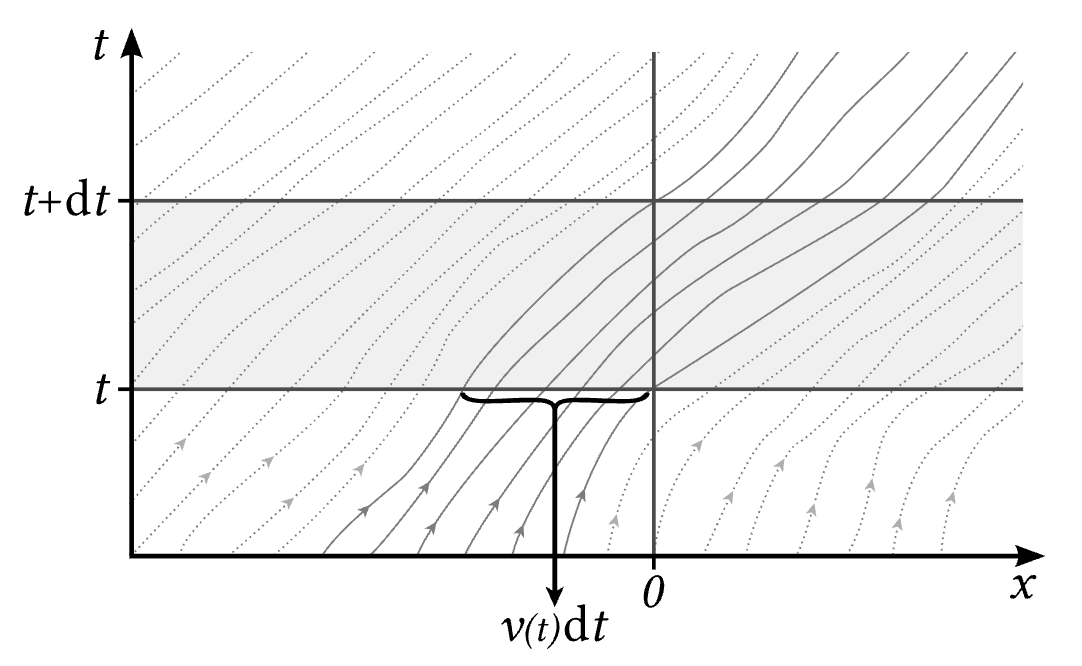
\includegraphics[width=1\linewidth]{Figures/prob_current_setup.png}
    \caption{Bohmian trajectories in the vicinity of the detector at $x=0$. Trajectories that cross the detector cover a distance of $\vec{v}(t)dt$ in a time interval $dt$. Image from \cite{paper:probability_current}.}
    \label{fig:probability_current_dt}
\end{figure}

This is essentially the same result as in canonical quantum mechanics, however we're now dealing with a physical justification for approaching this problem. What still has to be taken into account is the notion of cross the detector - it's perfectly possible for a bohmian trajectory to cross the detector twice. In these cases, the first crossing is usually taken into account, which is called \textbf{truncated current} in literature. Further this approach is readily generalizable to 3 dimensions, and detector shapes $\vec{r}_{\text{path}}$ of any kind.
\\\\
So far in our discussion, potentials in the pathway of the particle are not handled, nor is the modeling of the detector itself ignored, however when including these, the conclusions are generally the same:

\fbox{%
  \begin{minipage}{0.45\textwidth}
  The probability density of the arrival time $t$ at a detector $\vec{r}_{\text{detector}}$ is given by:
    \begin{align}
    \label{eq:continuitity_1}
    \Pi(t) = - j(\vec{r}_{\text{detector}}, t)
    \end{align}
    iff the bohmian trajectories are strictly positive to one direction across the detector.
  \end{minipage}%
}

In the discussed setup of a particle in free fall across a barrier, this is guaranteed to occur because the linear gravitational potential will always pull a particle down to the negative real axis. Further, by employing finetuned \textbf{complex absorption potentials} below the detector, we can ensure that no reflections to the positive directions occcur when simulating the experiment. In other words, even though no general POVM exists for modeling adequate probability currents that would correspond with the arrival time at the detector \textit{in general}, in highly specific setups like ours, and by employing adequate numerical techniques, it's still possible to produce meaningful physical results.

\subsubsection{Arrival Time for free-falling particles in low energy regimes}

Thus far, we held a general discussion about the arrival time. The discussion will now shift towards analysis of the physically realizable setup proposed in the introductory section of this study: a particle at rest is dropped in free fall onto a \textbf{delta barrier} at the origin, with a detector place below the origin at a distance $z=-L$ (see setup in figure \ref{fig:1d_setup} on page \pageref{fig:1d_setup}.
\\\\
The Hamiltonian of this setup is given by:

\begin{align}
i\hbar \frac{\partial}{\partial t} \psi(z,t) &= -\frac{\hbar^2}{2m} \frac{\partial^2}{\partial z^2} \psi(z,t) \notag \\&+ \left( \gamma \delta(z) + mgz \right) \psi(z,t)
\end{align}

The length and energy scales of the problem are well-known in literature:

\begin{align}
    \ell_0 = \sqrt[3]{\frac{\hbar^2}{2m^2g}}, \quad E_0 = mg\ell_0, \tag{2}
\end{align}

To make anysis of such a system easier, consider the introduction of the following dimensionless quantities:

\begin{align}
    z' = \frac{z}{\ell_0}, \quad t' = \frac{E_0}{\hbar} t, \quad \gamma' = \frac{\gamma}{E_0 \ell_0}. \tag{3}
\end{align}

 which after setting $\hbar=2m=\frac{g}{2}=1$, and substituting $\psi \rightarrow \psi'(z', t') = \sqrt{l_0} \space \psi(l_0 z', \frac{\hbar}{E_0}t')$ one gets:

\begin{align}
    i \frac{\partial}{\partial t} \psi(z,t) &= -\frac{\partial^2}{\partial z^2} \psi(z,t) \notag \\&+ \left( \gamma \delta(z) + z \right) \psi(z,t)
\end{align}

We now focus on the major analytical results proclaimed By Siddhant D. in \cite{siddhant:paper}, which calculates the probability current at a plane $z=-L$ through a delta barrier, by assuming far-field detectors ($L >> 1$), stationary-phase of the wave function, amd a low kinetic energy ($z_0$ is small, ie the particle is dropped from a low height). The solution is an approximate solution using well known Green's function solutions to the posed problem, and making assumptions as to the real part of the associated Propagators when solving the Green's function. The result of the cited paper are summarized in the following box:

\fbox{%
  \begin{minipage}{0.45\textwidth}
  \begin{align}
    \Pi_\gamma(\tau) &= -J_z(-L, \tau) \\ &\approx \frac{2 \tau \left| \hat{\psi}(L + \tau^2) \right|^2}{1 + (2\pi\gamma)^2 \operatorname{Ai}^4(-L - \tau^2)}
\end{align}
  \end{minipage}%
}

where $\gamma$ is the barrier strength (required to be small in this setup), and $L$ the distance of the detector from the origin, below the origin, and  $\hat{\psi}(E)$ is the \textit{Airy Transformed} of \psi_0:

\begin{align}
\hat{\psi}(E) = \left( 2 \sigma \sqrt{\pi} \right)^{1/2} 
\exp \left[ \frac{\sigma^2}{2} \left( \frac{\sigma^4}{6} + z_0 - E \right) \right] 
\times \\ \operatorname{Ai} \left( \frac{\sigma^4}{4} + z_0 - E \right),
\end{align}

and $\psi_0$ is a generic normalized Gaussian function of width $\sigma$, centered at $z_0$:

\begin{align}
    \psi(z, 0) = \frac{1}{\sqrt{\sigma} \sqrt{\pi}} \exp \left[ -\frac{(z - z_0)^2}{2\sigma^2} + i v_0 (z - z_0) \right]
\end{align}

This analytical result will be analysed with numerical methods later in this paper.\\\\
Note that this analytical solutions is only possible because of the delta potential setup, which is principle is not a realistic barrier. Realistic barriers are usually gaussian, which makes them impossible to solve analytically, especially with the linear gravitational potential component in the Hamiltonian.

\subsubsection{More on Probability Densities}

The probability current $J$ of the wave function $\Psi$ of spinless particles of mass $m$ in 1D is defined as:

\begin{align}
J &= \frac{\hbar}{2mi} \left( \Psi^* \partial_x \Psi - \Psi \partial_x \Psi^*  \right) \\
&= \frac{\hbar}{m} \Im \left( 
\Psi^* \partial_x \Psi \right)
\end{align}

In 3D, this generalizes to:

\begin{align}
\vec{J} &= \frac{\hbar}{2mi} \left( \Psi^* \nabla \Psi - \Psi \nabla \Psi^*  \right) \\
    &= \frac{\hbar}{m} \Im \left( \Psi^* \nabla \Psi \right)
\end{align}

For spin-S particles, the probability current obtains an extra field potential term, and a spin-component term, after substituting $\hat{\vec{p}} = -i\hbar \nabla$:

\begin{align}
\label{eq:spin-s}
\vec{J} &= \frac{1}{2m} \left[ \left( \Psi^* \space \hat{\vec{p}} \space \Psi - \Psi \space \hat{\vec{p}} \space \Psi^* \right) 
- 2q \space \vec{A} \space |\Psi|^2 \right]
\end{align}

For the purposes of this paper, neutral particles will be analyzed, hence $\vec{A}=0$. The current is sometimes written with the curl of spinor coupling, which is ignored in this text.

\subsection{Tunneling Time}

In the Bohmian Mechanical picture, tunneling time through a barrier is adequately defined due to the nature of \textbf{Bohmian trajectories}, and follows the same argument as for the arrival time in the previous section. Consider the setup as seen in figure \ref{fig:bohmian-tunneling}, where a normalized gaussian wave packet $\psi_0$ approaches a potential $V_0$.

\begin{figure}
    \centering
    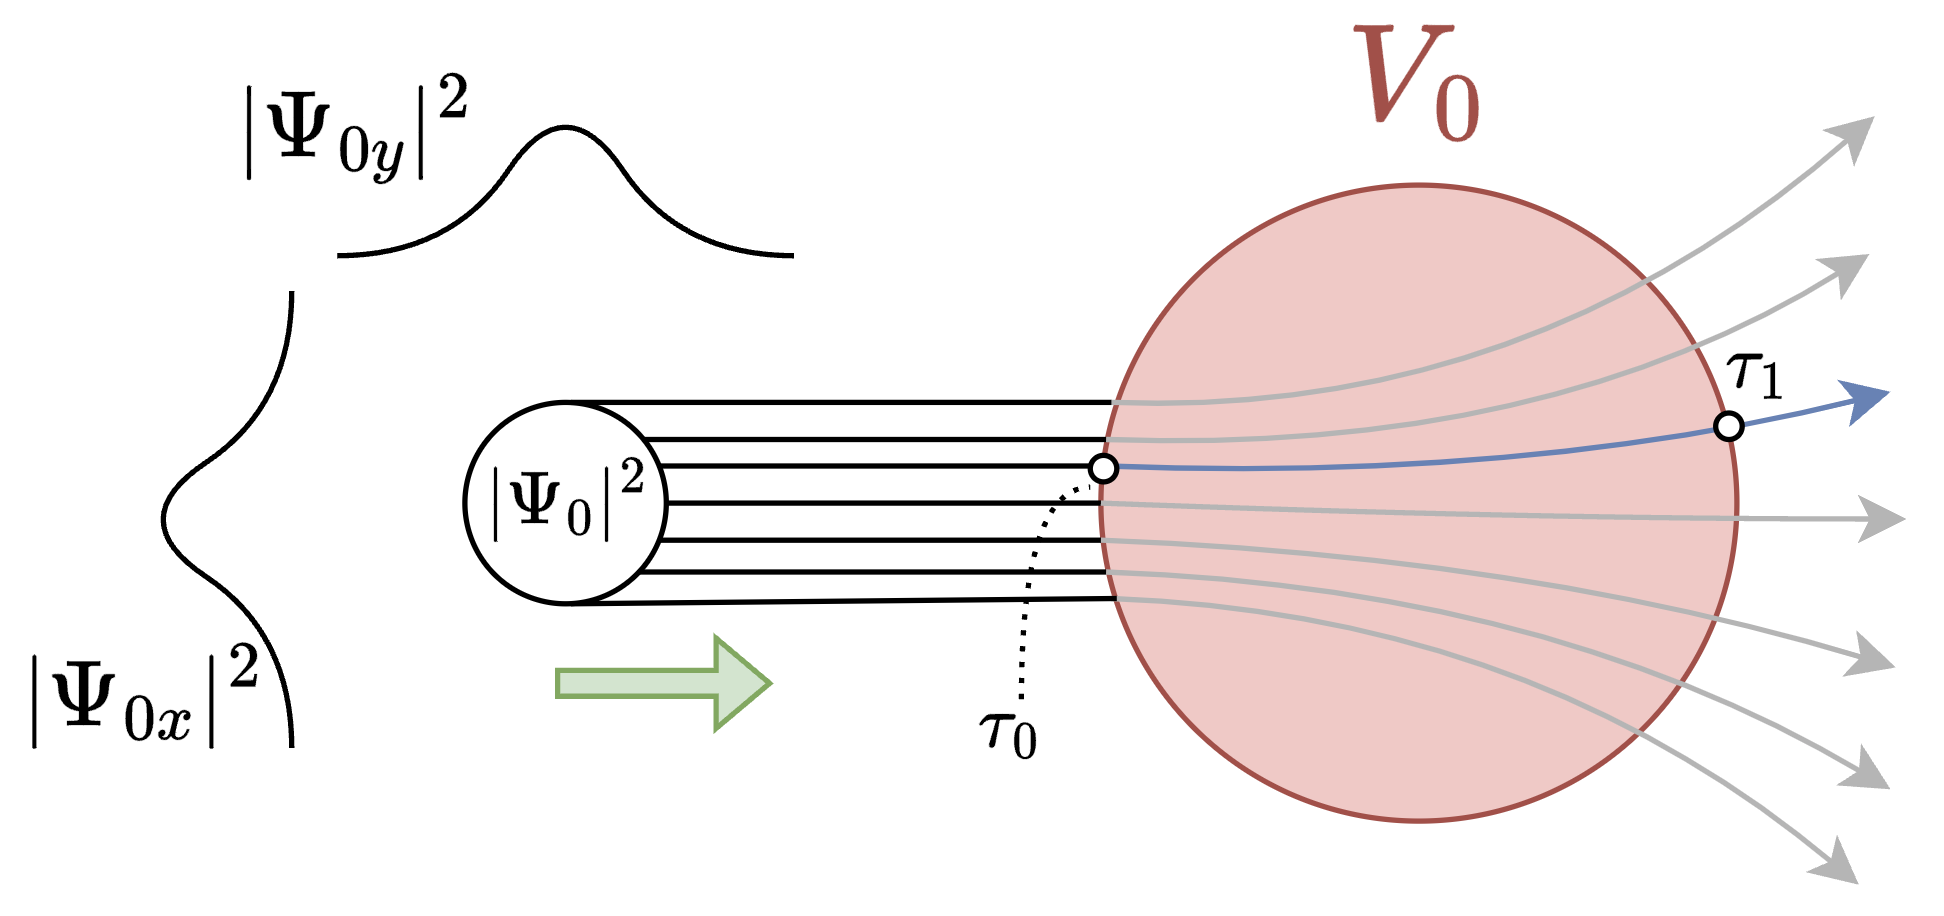
\includegraphics[width=1\linewidth]{Figures/tunneling_time_bohm.png}
    \caption{The tunneling time on Bohmian trajectory is defined as $\tau_1 - \tau_0$, respectively the time of entering and exiting the barrier, in case the boundaries of the barrier are well-defined.}
    \label{fig:bohmian-tunneling}
\end{figure}

Consider a Bohmian trajectory $\vec{Q}(t)$, which tunnels through the barrier of strength $V_0$. The tunneling time of this trajectory equals to $\tau_{Q} = \tau_1 - \tau_0$, at least \textbf{if the boundary of the barrier is well-defined}. In the discussion section of this paper, it shall be discussed how gaussian barriers have a not well-defined barrier, making the notion of tunneling time inherently ambiguous in the Bohmian picture. In any case, the average tunneling time of a quantum particle is the average tunnel time of N such Bohmian trajectories, which have been initialized in according to the wave function density distribution $|\psi_0|^2$:

\begin{align}
    \tau_t = \frac{1}{N} \sum_{i=0}^{N} \tau_{1}^{(i)} - \tau_{0}^{(i)}
\end{align}

It's important to emphesize that Bohmian trajectories are derived from the probability current $\vec{j}$, hence for adequate results, \textit{first crossing} of the barrier, and the first exit of the barrier, ought to be brought into consideration. In other words, backflow ought to be eliminated at the tiem window of tunneling. Numerically this can be solved by setting up complex absorbing potentials around the edges of the simulated domain, or stopping the simulation before the particle has significantly reached the edges of the simulation.

\subsection{Larmor Spin Precession And Larmor Clocks}
\label{ap:larmorspinprecession}

A classical electromagnetic result is that when a dipole is put into a uniform magnetic field $B_0$, then the dipole will start precessing at the \textbf{Larmor frequency} due to the torque exerted on the dipole moment. This quantity is given by

\begin{align}
    \omega_L = \gamma B_0.
\end{align}

This classical result applies to dipoles produced by quantum mechanical spin-$\frac{1}{2}$ particles. For electrons, $\gamma_e=-\frac{e}{2m_e}g_e$, with $g_e \approx2$, the electron g-factor, and $m_e$ the electron mass. For nuclei, $\gamma_N = \frac{e}{2 m_p}g$, with g the nuclear g-factor, and $m_p$ the proton mass. The main idea discussed in this sector is the retrieval of the \textbf{tunneling time $\tau_t$} from the spin precession.
\\\\
Consider a Hamiltonian for a spin-$\frac{1}{2}$ particle with a spin potential component:

\begin{align}
    \hat{H} = -\frac{\hbar^2}{2m} \nabla^2 - \vec{\sigma} \cdot \vec{B}
\end{align}

With $\vec{\sigma}$ the Pauli Spin Matrix vector. For simplicity consider a two dimension setup, with the $\vec{B}$ pointing in the positive z-direction. This simplies the Hamiltonian to

\begin{align}
    \begin{align}
    \hat{H} = -\frac{\hbar^2}{2m} \nabla^2 - \sigma_zB_z
\end{align}

Have a particle $\Psi$ prepared in some arbitrary superposition of spin up $\psi_{\uparrow}$ and spin down $\psi_{\downarrow}$, and assume $\Psi$ to be normalized in the usual fashion:

\begin{align}
    \Psi = \begin{pmatrix}
\psi_{\uparrow}(x,y,t) \\[6pt]
\psi_{\downarrow}(x,y,t)
\end{pmatrix}
\end{align}

As the particle will now evolve over time, the expectation values for Pauli Spin matrices $\langle \sigma_x\rangle$ and $\langle \sigma_y\rangle$ can be calculated,

\begin{align}
 \langle \sigma_x\rangle &= \langle \Psi | \sigma_x | \Psi \rangle\\
&= \frac{\hbar}{2}  \iint \begin{pmatrix}
\psi^*_{\uparrow}(x,y,t) \space \psi^*_{\downarrow}(x,y,t)
\end{pmatrix} \begin{pmatrix}
0 && 1\\ 1 && 0
\end{pmatrix} \notag \\ &\begin{pmatrix}
\psi_{\uparrow}(x,y,t) \\[6pt]
\psi_{\downarrow}(x,y,t)
\end{pmatrix} 
\end{align}

, equivalently for $\langle \sigma_y\rangle$ with $\sigma_y = \frac{\hbar}{2} \begin{pmatrix}
0 && -i\\ i && 0
\end{pmatrix}$. This returns the following two equations for the expectation values:

\begin{align}
    \langle \sigma_x\rangle
=
\iint \Bigl[
 \psi_{\uparrow}^\ast(x,y)\,\psi_{\downarrow}(x,y)
 \;\notag \\+\;
 \psi_{\downarrow}^\ast(x,y)\,\psi_{\uparrow}(x,y)
\Bigr]
\,d^2r,
\\
\langle \sigma_y\rangle
=
\Im \iint \Bigl[
 \psi_{\uparrow}^\ast(x,y)\,\psi_{\downarrow}(x,y)
 \;\notag  \\-\;
 \psi_{\downarrow}^\ast(x,y)\,\psi_{\uparrow}(x,y)
\Bigr]
\,d^2r
\end{align}

When dealing with a discretized simulation of partial the TDSE, the spin quantities are obtained by summsing complex amplitudes of the wavefunctions in the following way:

\begin{align}
    \langle \sigma_x\rangle
&\approx
\Delta x\,\Delta y 
\,\sum_{i,j}\,
\Bigl[\,
 \psi_{\uparrow}^\ast(x_i,y_j)\,\psi_{\downarrow}(x_i,y_j)
 \\
 &+
 \psi_{\downarrow}^\ast(x_i,y_j)\,\psi_{\uparrow}(x_i,y_j)
\Bigr],
\end{align}
and similarly for $\langle \sigma_y\rangle$, with $\Delta x$ and $\Delta y$ the grid size of the discretization.
\\\\
In a weak magnetic barrier, one may expect a shift in phase, accrued inside the barrier region, and hence the precession angle can be approximated by

\begin{align}
\Theta(t) \approx 
\tan^{-1}\!\Bigl(\,
\frac{\langle \sigma_y\rangle}{\langle \sigma_x\rangle}
\Bigr).
\end{align}

The time returned by the \textbf{Larmor Clock} is now a dynamically derived quantity of the time spent in the barrier, given by

\begin{align}
    \label{eq:dwell_123}
    \tau_{tunneling} = \frac{\Delta\Theta}{\gamma B_0} = \frac{\Delta\Theta}{\omega_L}
\end{align}

, which corresponds to Bütticker weak-field explession of the larmor clock \cite{Buttiker1983LarmorClock}. This approximation has been derived by Bütticker for square wells, but he has demonstrated that the approximation holds for any symmetric barriers. In this study we're using the circular square well, and the Gaussian barrier, both of which are symmetrically placed at the origin. Bütticker original formula states that $\tau = \sqrt{\tau_p^2 + \tau_t^2}$, where $\tau_p$ is the spin precession in the xy plane on the Bloch sphere, whereas $\tau_t^2$ is the time it took for the spin states to start mixing - the transversal spin precession. In this study, both symmetric barrieirs, and weak ones are considered, quaranteeing that the spin states are not mixing. Bütticker's Larmor Clock has been critiqued, with a rebuttal posed in \cite{LeavensAers1988LocalClock}. In 2021, another rebuttal came to the forefront by \cite{Sokolovski2021}, which corresponds with findings in this study.
\\\\
In this study, the \textbf{larmor clock} and \textbf{Bohmian tunneling time} are compared and discussed.
\\\\
Most theory regarding the physics has been discussed and presented. What follows is a series of section regarding numerical simulations of quantum systems.

\subsection{The Split Operator Method}

This section is concerned with the theoretical aspects of simulation a time dependent schrödinger equation in a discretized fashion, and in particular of a well known method that is both fast and accurate on limited hardware, the \textbf{Split Operator Method}, which is a different name for the Strange Splitting method.
\\\\
Consider the general case of numerically solving a linear equation

\begin{align}
    \dot{y} = L_1 (y) + L_2(y)
\end{align}

where $L_1$ and $L_2$ are linear operators. With associated solution:

\begin{align}
    y = e^{(L_1 +L_2)t} y_0
    \label{eq:basicsolution}
\end{align}

If $L_1$ and $L_2$ commute, then by exponential laws, equation \ref{eq:basicsolution} simplifies to

\begin{align}
    y = e^{L_1t}e^{L_2t}  y_0
    \label{eq:basicsolution}
\end{align}

If $L_1$ and $L_2$ don't commute, then by using Baker-Campbell-Hausdorff (BCH) formula, 

\begin{align}
    e^{(\hat{X}+\hat{Y})} = e^{\hat{X}} e^{\hat{Y}} e^{\frac{1}{2}[\hat{X}, \hat{Y}]} + \dots
\end{align}

one can still split up the solution, with an error $\bigO(t^2)$:

\begin{align}
    y = e^{(L_1 +L_2)t} y_0 = e^{L_1t}e^{L_2t} y_0 + \bigO(t^2) 
    \label{eq:extended}
\end{align}

One may now solve solve the solution iteratively by taking timestep $\Delta t$, and applying the linear operators one after another:

\begin{align}
    \tilde{y}_1 = e^{L_1 \Delta t} y_0\\
    y_1 = e^{L_1 \Delta t} \tilde{y}_1\\
    \tilde{y}_2 = e^{L_1 \Delta t} y_1\\
    y_2 = e^{L_1 \Delta t} \tilde{y}_2
\end{align}

The error can be reduced to $\bigO(t^3)$ by using Taylor Expansions and comparing error terms, whose details are out of scope of this text. The solution involves taking taking \textit{half steps} for either one of the linear operators. An iteration looks as follows:

\begin{align}
    \tilde{y}_1 = e^{L_1 \frac{\Delta t}{2}} y_0\\
    \bar{y}_1 = e^{L_2 \Delta t} \tilde{y}_1\\
    y_1 = e^{L_1 \frac{\Delta t}{2} } \bar{y}_1\\
    \tilde{y}_2 = e^{L_1 \frac{\Delta t}{2}} y_1\\
    \bar{y}_2 = e^{L_2 \Delta t} \tilde{y}_2\\
    y_2 = e^{L_1 \frac{\Delta t}{2}} \bar{y}_2
\end{align}

This process is called \textbf{Strange Splitting}, and it can be easily applied to the time-dependent Schrödinger equation . Consider a wave function $\Psi(\vec{r}, t+dt) = \Psi(t+dt)$ (written without position to save space) over time, in single iteration timesteps $dt$ and a Hamiltonian $\hat{H} = \hat{H}_{kin} + \hat{H}_{pot} = \hat{T} + \hat{V}$. The Strange splitting looks as follows for this method:

\begin{align}
    \Psi(t+dt) &= exp\left( -\frac{i}{\hbar} \hat{H} dt \right) \Psi(t) \\
    &= e^{-\frac{i}{\hbar} \hat{H}_{pot} dt} e^{ -\frac{i}{\hbar} \hat{H}_{kin} dt } \Psi(t) + \bigO(t^2)\\
    &= e^{-\frac{i}{\hbar} \hat{H}_{pot} \frac{dt}{2}}  e^{ -\frac{i}{\hbar} \hat{H}_{kin} dt } e^{-\frac{i}{\hbar} \hat{H}_{pot} \frac{dt}{2}} \Psi(t) \notag\\ &+ \label{eq:strangesplitting} \bigO(t^3)
\end{align}

The Split Operator Method is the name given the process where equation \ref{eq:strangesplitting} can be quickly and efficiently iterated upon using Fast Fourier Transforms (FFT). In quantum mechanics, the fourier transformation of the wavefunction transforms it into \textbf{momentum space}, allowing the momentum-space transformed wave function to be efficiently multiplied by $e^{ -\frac{i}{\hbar} \hat{H}_{kin} dt }$. The whole process involves multiplying the wave function's complex amplitudes by the Strange Splitted Hamiltonian in equation \ref{eq:strangesplitting}, with FFT and iFFT inbetween the \textit{potential half steps}. The Split Operator Method looks as following:

\begin{align}
\Psi(z)|_{t} \\
& \xrightarrow{\text{Potential Half Step}} \Psi(z) \times  e^{-\frac{i}{2 \hbar} \hat{V}(z) dt} \\
& \xrightarrow{\text{FFT}} \tilde{\Psi}(k) \\
& \xrightarrow{\text{Kinetic Step}} \tilde{\Psi}(k) \times e^{ -\frac{i}{\hbar} \hat{H}_{kin} dt } \\
& \xrightarrow{\text{Inverse FFT}} \Psi(z) \\
& \xrightarrow{\text{Potential Half Step}} \Psi(z) \times  e^{-\frac{i}{2 \hbar} \hat{V}(z) dt} \\
\Psi(z) |_{t+dt}
\end{align}

Since the FFT and iFFT have been adequately optimised, the split operator method is not only accurate, but incredibly fast.
\\\\
The Split Operator Method generalizes readily to multiple dimensions, although for this 2 dimension or 3 dimensional FFT ought to be used before applying the kinetic step. Furthermore, this numeric methods requires that the grid space be small enough, such that the discretized momenta in k-space are adequately applied, depending on the barriers and potentials present in the setup.
\\\\
The Split Operator Method is also easily applied to simulations of spin-$\frac{1}{2}$ particles, where $Psi$ is then represented by a Pauli spinor. This is discussed in the next section.

\subsection{Yoshida's Composition Method - Fourth Order Accuracy}

For some applications and simulations, the local errors of the Strange splitting method of order $dt^3$ are too big, and fourth-order accurate methods are desirable. Y. Yoshida \cite{Yoshida1990} developed a method for constructing higher-order symplectic integrators, composed of several second-order steps. For completion it's worth mentioning that the 4th order extension of the Strange method is attributed to \textbf{Forest-Ruth}. In either case, a second order step looks like:

\begin{align}
    U(t) = e^{-i\frac{t}{2}\hat{V}} e^{-it\hat{T}} e^{-i\frac{t}{2}\hat{V}} 
\end{align}

Yoshida's method prescribes the following composition:

\begin{align}
    U_4(\Delta t) = \space &U(p_1 \Delta t) \, U(p_2 \Delta t) \, U(p_1 \Delta t)
\label{eq:composition}
\end{align}

Where the coefficients $p_1$ and $p_2$ are to satisfy

\begin{align}
    2p_1 + 2p_2 = 1\\
    2p_1^3 + y_2^3 = 0
\end{align}

and are chosen such that the leading error terms cancel. This method produces symplectic integrators (volume and surface preserving in phase space). A common choice in literature is:

\begin{align}
p_1 = \frac{1}{2-2^{1/3}}, \quad p_2 = -\frac{2^{1/3}}{2-2^{1/3}}
\end{align}

This construction cancels the third-order error terms, yielding a local error of order \(\Delta t^5\) and a global error scaling as \(\Delta t^4\). The fourth order Yoshida's method will be used to assess the adequacy of employed computation models for arrival and tunneling time.

\paragraph{Note: On Yoshida Method}  

The previously discussed method can be further extended to 6th and 8th order accuracy, using Yoshida's Recursive method. The $\bigO(dt^8)$ contains 15 Strange steps with carefully chosen coefficients to cancel out higher order errors. This is out of scope of this study, but could be conducted for further testing to ensure high accuracy of leading terms.

\subsection{Complex Absorption Potentials}
\label{sec:cap}

As mentioned at the start of this section, to ensure positive probability current flow in the studied free fall setup beyond Gaussian potentials, it's vital to absorb the wave function at the edges of the simulated domain, and ensure no reflections back up the detector, causing backflow. A first attempt to absorbing the wave function uses Gaussian attenuation masks at about 30\% of the edges of the simulation. This approaches causes a lot of reflections. The state-of-the-art approach towards absorbing wave functions is by sing Complex Absorption Potentials, which are of the form

\begin{align}
    -iW(\vec{r}),
\end{align}

which is added to the Hamiltonian

\subsubsection{Polynomial Complex Absorbing Potential (CAP)}
\label{subsec:poly_cap}

A simple power–law CAP that turns on smoothly inside an
absorbing layer of width \(L\) at each box edge:
\begin{align}
W(x)=
\begin{cases}
\displaystyle 
\eta\bigl(\xi/L\bigr)^{n}, & \xi>0,\\[4pt]
0, & \xi\le 0,
\end{cases}
\\ \qquad\text{with}\quad 
\xi=
\begin{cases}
x_{\min}+L-x,&x<x_{\min}+L,\\
x-(x_{\max}-L),&x>x_{\max}-L,
\end{cases}
\end{align}

Here  
\(\eta>0\) is the strength,  
\(n\ge 2\) the even polynomial order,  
and \(L\) the physical thickness of the absorbing strip.
Increasing \(n\) steepens the profile and reduces low‑energy
reflection roughly as \(R\!\propto\!L^{-(2n-2)}\).
(Adapted from Feit, Fleck \& Steiger - \cite{feit1982spectral}.)

In literature, plenty more CAPs can be found, like Gaussian CAPS (didn't work well the setup of this study), Manolopoulos Transmission‑Free CAP (TFAP), Riss–Meyer Reflection‑Free CAP (RF‑CAP), or Smooth Exterior‑Scaling (SES) CAP. These have been quickly tested and asssesed. It has been concluded that for the use case of this study, the polynomial CAP works very well, when the parameters are well chosen.

\subsection{Spectral Derivation}

In the spectral method, spatial derivatives are computed by transforming the wavefunction into Fourier space, where differentiation becomes a simple multiplication operation. Suppose $\psi(x, y)$ is defined on a discrete grid. Taking its Fast Fourier Transform (FFT) yields $\tilde{\psi}(k_x, k_y)$, the representation in wave number space. Differentiation with respect to $x$ and $y$ then becomes:

\begin{align}
\frac{\partial \psi}{\partial x} \longleftrightarrow i k_x \tilde{\psi}(k_x, k_y),\\
\frac{\partial \psi}{\partial y} \longleftrightarrow i k_y \tilde{\psi}(k_x, k_y)
\end{align}

After this multiplication, applying the inverse FFT retrieves the spatial derivatives:

\begin{align}
\frac{\partial \psi}{\partial x} = \mathcal{F}^{-1} \left[ i k_x \tilde{\psi}(k_x, k_y) \right], \\
\frac{\partial \psi}{\partial y} = \mathcal{F}^{-1} \left[ i k_y \tilde{\psi}(k_x, k_y) \right]
\end{align}

This approach is highly accurate for periodic or smoothly truncated domains and avoids the finite-difference approximations typically used in grid-based methods. Using spectral derivation was pivotal to computing Bohmian Trajectories for relative small grid-sized.

\subsection{1D Simulations}

In order to confront the analytical estimates with fully dynamical data, a one–dimensional time–dependent Schrödinger equation is solved on a finite spatial grid
\(
z\in[x_{\min},x_{\max}]
\)
using the split–operator propagator already introduced in the previous section. Only the elements specific to the present free-fall setup are summarized below.

\paragraph{Spatial discretization.}
The coordinate axis is discretized by a uniform mesh
\(
z_j = x_{\min}+j\,\Delta z,\; j=0,\dots,N_x-1
\)
with \(\Delta z=(x_{\max}-x_{\min})/N_x\).
Derivatives entering the kinetic phase factor are evaluated in momentum space through the discrete Fourier transform, \(k_j = 2\pi j /(N_x\Delta z)\), but in practice through the Fast Fourier Transform. Kinetic factors are calculated upfront for the discretized spatial grid, allowing for quick simulation times.

\paragraph{External potential.}
The total potential consists of a linear gravitational term, a tunable barrier at the origin, and an optional complex absorbing part,  
\begin{equation}
    V(z) \;=\; mgz\;+\;V_{\text{bar}}(z)\;-\;iW(z),
\end{equation}
where \(m=g=\hbar=1\) in the simulation’s natural units.

\paragraph{Barrier.}  
          Two barrier models are implemented in the simulation:
          \begin{align}
              V_\delta(z) &= \alpha\,
              \frac{\exp\!\bigl[-(z-z_0)^2/2\sigma^2\bigr]}
                   {\sqrt{2\pi}\sigma},
              &&\sigma=\tfrac12\Delta z,\tag{\textit{``delta''}}\\[4pt]
              V_g(z)      &= V_0\,
              \exp\!\bigl[-(z-z_0)^2/2\sigma^2\bigr],\tag{\textit{``gaussian''}}
          \end{align}
          where the first line approximates an ideal \(\delta\)-barrier by a narrow Gaussian whose width is tied to the grid spacing.
          
\paragraph{Absorber.}  
          At the simulation boundaries a complex absorbing potential \(W(z)\ge 0\) (or, equivalently, a multiplicative mask) suppresses unphysical reflections, enabling long propagation times with modest box sizes. Grid searches for the polynomial CAP are employed for the CAP's free parameters width (absorption layer width), $\eta$ (absorption), and $n$ (degree). See section \ref{subsec:poly_cap} on page \pageref{subsec:poly_cap} for more information. Making the simulation space large enough, employing a width of at least 30\% of that of the simulated space, together with a large ($\approx 10^3$), work exceedingly well at absorbing all but the most faint complex amplitudes of the wave function (order of $\approx 10^{-8}$).

\paragraph{Initial state.}
A minimum-uncertainty, normalized Gaussian packet is released from height \(z_0\) with mean momentum \(p_0\),
\begin{align}
    \psi(z,0) &=\frac{1}{(2\pi\sigma_0^2)^{1/4}}\\
              & \exp\!\Bigl[
                   -\frac{(z-z_0)^2}{4\sigma_0^2}
                   +\frac{i\,p_0}{\hbar}(z-z_0)
              \Bigr].
\end{align}

For all experiments conducted in this study, $p_0$ has been set to 0.
\\
\paragraph{Time stepping.}
For each interval \(\Delta t\) the state is advanced according to
\begin{align}
\psi(t+\Delta t) &=
e^{-\frac{i}{2\hbar}V\Delta t}\, \\
& \mathcal{F}^{-1}\!\bigl[e^{ -\frac{i\hbar k^2}{2m}\Delta t }\,
\mathcal{F}[\psi(t)]\bigr]\,
e^{-\frac{i}{2\hbar}V\Delta t},
\end{align}
or, when higher accuracy is desired, by the fourth-order Yoshida composition of these split steps.

\paragraph{Recorded observables.}
At each step we store the probability density \(|\psi(z,t)|^2\), the cumulative absorbed norm, and the raw complex amplitudes of the wave function using NumPy's 128-bit Complex Value Type.
The local probability current required for the arrival-time distribution per unit time is evaluated as
\begin{align}
j(z,t)=\dfrac{\hbar}{m}\,\Im\bigl[\psi^*(z,t)\,\partial_z\psi(z,t)\bigr].
\end{align}

All numerical data shown in the remainder of this work are obtained with the above scheme using \(N_x=2048\), \(\Delta t=10^{-3 }s\), and box limits \(x_{\min}=-40,\,x_{\max}=40\), in dimensionless units, unless stated otherwise.

\paragraph{Plotting.}
For plotting, the python library \textbf{matplotlib} is used.
\\\\

For 2-dimensionalal simulations of the same kind (without spin), the setup remains largely the same.

\subsection{2D Simulations with Spin}

\label{sec:spin-dynamics-2d}

The setup for modeling Gaussian spin-$\frac{1}{2}$ particles falling under free fall throughout a magnetic is modelled by propagating a two–component spinor  
\(
\Psi(\mathbf r,t)=
\bigl(\psi_\uparrow(\mathbf r,t),\,
       \psi_\downarrow(\mathbf r,t)\bigr)^{\!\mathsf T},
\quad
\mathbf r=(x,y),
\)
under a Hamiltonian that separates into kinetic and spin–dependent
potential parts,  
\begin{align}
    \hat{H} &=      \underbrace{\vphantom{\bigl|}\Bigl[-\dfrac{\hbar^{2}}{2m}
      \bigl(\partial_x^{2}+\partial_y^{2}\bigr)\Bigr]}_{\hat{T}\,\otimes\,\mathbbm \mathbb{1}_{2\times2} } \\
      &+\;
      \underbrace{\bigl[\,V_0(\mathbf r)\,\mathbbm 1_2
                      +V_B(\mathbf r)\,\sigma_z\bigr]}_{\hat{V}(\mathbf r)}
\end{align}
where  
\(V_0(\mathbf r)=mg\,y\) is the spin–independent gravitational term and  
\(V_B(\mathbf r)\) is a magnetic barrier that couples to the Pauli
matrix $\sigma_z$. With the barrier centered at, \((x_0,y_0)\), a Gaussian profile is used for modeling a physically realistic laser profile
\begin{align}
V_B^{(\text{G})}=V_0^{\text B}\exp[-(\rho/\sigma)^2/2],\\
\rho^2=(x-x_0)^2+(y-y_0)^2,
\end{align}
or, in the second situation, a hard–edged circular uniform magnetic field $B_0$. Both situations will be compared regarding the notion of tunneling time.

\paragraph{Split-operator step.}
At every time increment \(\Delta t\) the state is advanced by the
second–order factorization
\begin{align}
U(\Delta t)=
e^{-\frac{i}{2\hbar}V\,\Delta t}\;
e^{-\frac{i}{\hbar}T\,\Delta t}\;
e^{-\frac{i}{2\hbar}V\,\Delta t},
\end{align}
applied as  
\begin{align}
 &\Psi(\mathbf r,\,t+\Delta t)=
          U(\Delta t)\,\Psi(\mathbf r,t)
\end{align}
with
\begin{align}
 e^{-\frac{i}{2\hbar} \hat{V} \,\Delta t}\;=\;
   \begin{pmatrix}
      e^{-\frac{i}{2\hbar}(V_0+V_B)\,\Delta t} & 0 \\[6pt]
      0 & e^{-\frac{i}{2\hbar}(V_0-V_B)\,\Delta t}
   \end{pmatrix}\!,
\label{eq:V-matrix}
\end{align}

and  
\begin{align}
e^{-\,\tfrac{i}{\hbar}T\,\Delta t}
      =\exp\!\bigl[-\tfrac{i\hbar(k_x^2+k_y^2)}{2m}\Delta t\bigr]\mathbbm \mathbb{1}_{2\times2}
\end{align}after transforming to momentum space
\(
(k_x,k_y)=2\pi(j_x/N_x\Delta x,\,j_y/N_y\Delta y).
\)
The matrix in~\eqref{eq:V-matrix} acts pointwise in real space; its
diagonal form means that spin-up and spin-down amplitudes merely acquire
opposite phases, hence \textbf{no spin mixing occurs}, which would require keeping track of the Transversal Spin Precession of the Larmor clock, as proposed by the original Bütticker paper.

\paragraph{Explicit component-wise action.}
Writing out the full 2\(\times\)2 multiplication for the potential half
step makes the algorithmic structure transparent:
\begin{align}
\begin{pmatrix}\psi_\uparrow\\\psi_\downarrow\end{pmatrix}
\;\xrightarrow{\;V\;}\;
\begin{pmatrix}
  e^{-\frac{i}{2\hbar}(V_0+V_B)\Delta t}\,\psi_\uparrow \\
  e^{-\frac{i}{2\hbar}(V_0-V_B)\Delta t}\,\psi_\downarrow
\end{pmatrix}.
\end{align}
After the kinetic FFT step (common to both components) the same matrix
is applied once more, completing the single-time-step propagation.

\paragraph{Initial state and observables.}
The simulation starts from an equal superposition
\begin{align}
\Psi(\mathbf r,0)=\tfrac{1}{\sqrt2}\,
      \psi_0(\mathbf r)\,\bigl(1,1\bigr)^{\!\mathsf T}
\end{align}
with a minimum-uncertainty packet
\begin{align}
\psi_0 &= \left(2\pi\sigma^2\right)^{-1/2} \times \\ & \exp\left[ 
        -\frac{(\mathbf{r} - \mathbf{r}_0)^2}{4\sigma^2} 
        + \frac{i \mathbf{p}_0 \cdot (\mathbf{r} - \mathbf{r}_0)}{\hbar} 
        \right]
\end{align}
where $\mathbf{p}_0$ is set to zero in all discussed simulations in this study. At every stored step, the spin-resolved probabilities
\(P_{\uparrow,\downarrow}=|\psi_{\uparrow,\downarrow}|^{2}\) and raw complex amplitudes of the wave function are stored using NumPy's 128 bit complex number type.
\\\\
For 2D simulations, the number of memory required to complete a succesful iteration grows exponentially. A discretization of $Nx=Ny=512$ at a $\Delta t=0.01s$ for a space of $x,y \in \mathbb{R}^2 \quad \text{limited to} \quad [-20, 20]$ worked well for producing physically feasibly simulations. The explored free parameter space explored in this study is listed:

\begin{itemize}
    \item Magnetic Barrier Strength $B_0\in \{ 0.5,  \}$
    \item Magnetic Barrier Width - $\sigma=2$
    \item Magnetic Barrier Type - Gaussian and Hard-Edged Uniform Circle
    \item Number of steps = 300
    \item Drop height = 15 units
    \item Particle at rest, $p_{0x}=p_{0y}=0$
\end{itemize}

\subsection{General Workflow}

In this section, a brief overview of numeric workflows are laid out, such that it's better understood how to reproduce the resultes in the next section.
\\\\
First, Siddant Das \cite{siddhant:paper} low energy regime model for the arrival time distribution is compared with the setup numerical simulations.
\\\\
After this, the arrival time density for 1-dimensional simulations is analyzed for different barrier strengths, different drop heights, and the tunneling behavior is characterized. For 1 dimension simulations, the calculated space across 50+ simulations can be held into memory. The arrival time results generally translate to two and even three dimensional results, if spin is excluded from the calculation.
\\\\
Next up, tunneling time is analysed in the \textbf{Larmor Clock} theory and Bohmian Theory. For this, two magnetic barrier types are tested at different strengths (circular and Gaussian magnetic uniform barriers). The simulation is ran for 3 seconds, until the wave function hits the barrier. The simulated setup can be seen in figure \ref{fig:1d_setup} on page \pageref{fig:1d_setup}. For two dimensional modeling and layering, each simulation data needs to be stored separely on file ($\approx$ 6.5 $Gb$ per file), requiring about 450Gb in storage for storing all 2D simulations made in this study. This storage space is readily available in the commercial laptop range. A single 2d simulation run takes 15-25 minutes, depending on available CPU and RAM resources, and simulation parameters. The general workflow for gathering quantities across many simulations is depicted in figure \ref{fig:general-workflow}.

\begin{figure}
    \centering
    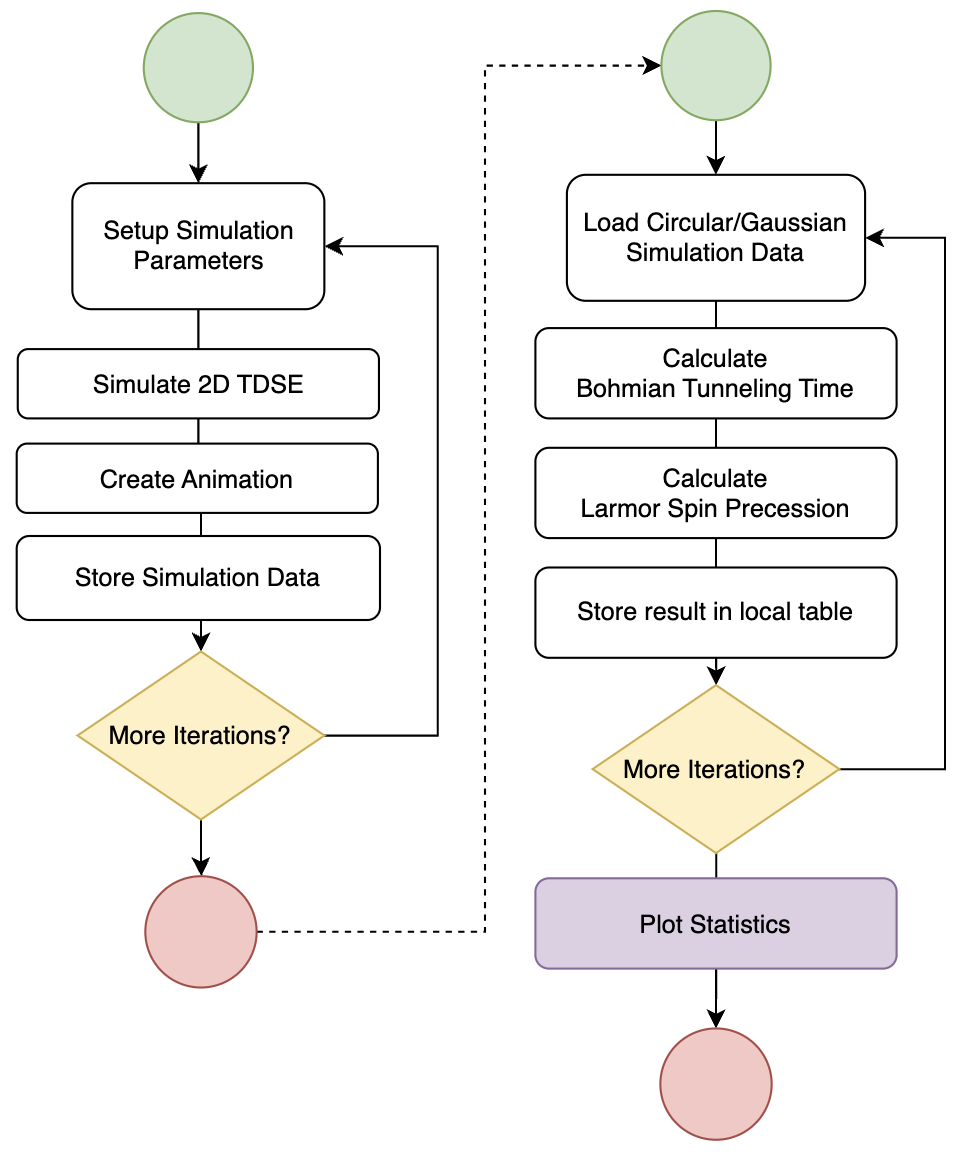
\includegraphics[width=1\linewidth]{Figures/sim_steps.png}
    \caption{General process for arrival time and tunneling time statistics}
    \label{fig:general-workflow}
\end{figure}

